%% ma: L12-B05-0021
%% lop: 12
%% chuong: 1
%% bai: 5
%% dang: 12.5.8
%% loai: TLN
%% muc: VD
%% dap_an: "21"
%% nguon: "(NBV)-ĐỀ SỐ 11-MỖI NGÀY 1 ĐỀ THI 2025.pdf (D11, MỖI NGÀY 1 ĐỀ - Đề số 11), Phần III Câu 6 (THPT Lê Xoay - Vĩnh Phúc 2025)"
%% kien_thuc: "Bài 5 (tối ưu bằng đạo hàm, tổng hai căn thức), Toán 10 Bài 6 (định lí Pythagore)"
%% trang_thai: chinh-thuc
%% ghi_chu: "Đáp án gốc 21 đúng (sympy: nhỏ nhất tại x = 5, t = 5 căn 5 / 6). Hình dựng lại từ số liệu: d là đường thẳng ngang, A cách d 10 km phía đất ướt, C cách d 10 km phía đất khô, AC = 5 căn 41 km; không theo tỉ lệ thực. Cùng ý tưởng với L12-B05-0011 và L12-B05-0012 (tối ưu thời gian/quãng đường qua hai môi trường, tổng hai căn thức), nhập vào dạng đã duyệt."
\begin{ex}
Một người cưỡi ngựa xuất phát từ $A$ đi đến $C$. Điểm $A$ nằm trong vùng đất ướt nên vận tốc của ngựa khi đi trong vùng này là $12$ km/h. Điểm $C$ nằm trong vùng đất khô hơn nên vận tốc của ngựa khi đi trong vùng này là $24$ km/h. Hai phần đất này giáp nhau bởi một đường thẳng $d$ đi qua trung điểm của $AC$ và khoảng cách từ $A$ và $C$ đến đường thẳng này đều bằng $10$ km.
\begin{center}
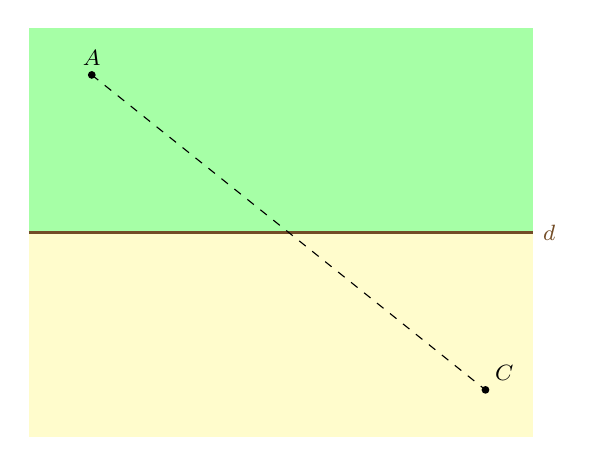
\begin{tikzpicture}[scale=.2]
  \fill[green!35] (-3,0) rectangle (29,13);
  \fill[yellow!20] (-3,-13) rectangle (29,0);
  \draw[thick,brown!60!black] (-3,0)--(29,0) node[right,font=\footnotesize] {$d$};
  \coordinate (A) at (1,10);
  \coordinate (C) at (26,-10);
  \draw[dashed] (A)--(C);
  \fill (A) circle (7pt) node[above,font=\footnotesize] {$A$};
  \fill (C) circle (7pt) node[above right,font=\footnotesize] {$C$};
\end{tikzpicture}
\end{center}
Biết $AC=5\sqrt{41}$ km, thời gian ít nhất để đi từ $A$ đến $C$ là $t=\dfrac{a\sqrt5}b$ giờ ($a,b\in\mathbb N^*$, $a,b$ nguyên tố cùng nhau). Tính $T=3a+b$.
\shortans{21}
\loigiai{Gọi $H$, $K$ là chân đường vuông góc kẻ từ $A$, $C$ đến $d$. Vì $d$ đi qua trung điểm của $AC$ và $AH=CK=10$ nên $HK=\sqrt{AC^2-(AH+CK)^2}=\sqrt{25\cdot41-400}=25$ km.

Giả sử người đó đi đến điểm $M\in d$ với $HM=x$ $(0\le x\le25)$. Thời gian đi là
\[f(x)=\dfrac{\sqrt{x^2+100}}{12}+\dfrac{\sqrt{(25-x)^2+100}}{24}.\]
$f'(x)=\dfrac1{12}\cdot\dfrac{x}{\sqrt{x^2+100}}-\dfrac1{24}\cdot\dfrac{25-x}{\sqrt{(25-x)^2+100}}$; $f'(5)=\dfrac1{12}\cdot\dfrac5{\sqrt{125}}-\dfrac1{24}\cdot\dfrac{20}{\sqrt{500}}=0$, và $f'$ đồng biến nên $x=5$ là nghiệm duy nhất, $f'<0$ khi $x<5$, $f'>0$ khi $x>5$.

Do đó $\min f=f(5)=\dfrac{\sqrt{125}}{12}+\dfrac{\sqrt{500}}{24}=\dfrac{5\sqrt5}{12}+\dfrac{10\sqrt5}{24}=\dfrac{5\sqrt5}{6}$. Suy ra $a=5$, $b=6$, $T=3\cdot5+6=21$.}
\end{ex}
